% 导言区
\documentclass{ctexart}%ctexbook, ctexrep

%\usepackage{ctex}

\usepackage{graphicx}
\graphicspath{{figure/},}%图片在当前目录下的figure文件夹中

% 标题控制(caption、bicaption等宏包)
% 并排与子图表(subcaption、subfig、floatrow等宏包)
% 绕排(picinpar、wrapfig等宏包)

% 正文区(文稿区)
\begin{document}
	\LaTeX{}中的插图\ref{fig-lion}:
	\begin{figure}[htbp]
		\centering
		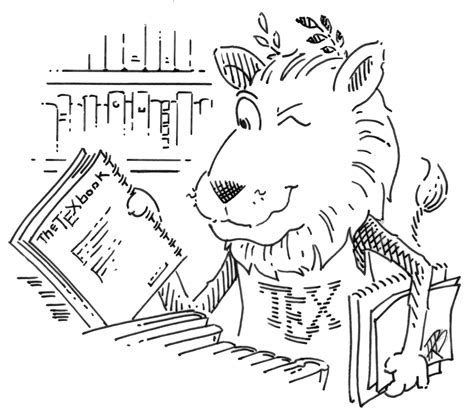
\includegraphics[scale=0.3]{lion}
		\caption{\TeX 系统的吉祥物---小狮子}\label{fig-lion}
	\end{figure}	
    
    桂林山水甲天下(图\ref{fig-guilin})
    \begin{figure}[htbp]
    	\centering
    	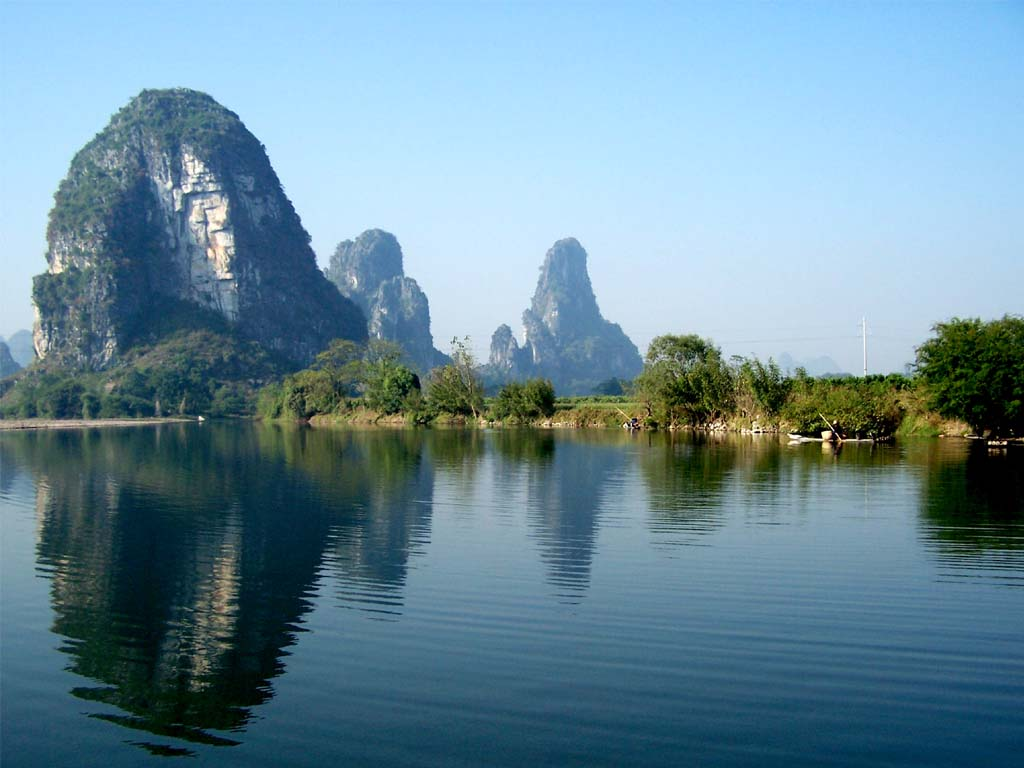
\includegraphics[scale=0.3]{guilin}
    	\caption{\TeX 桂林风景美如画}\label{fig-guilin}
    \end{figure}
    
    \LaTeX{}中的表格\ref{tab-chengji}:
    \begin{table}[htbp]
    	\centering
    	\caption{考试成绩}\label{tab-chengji}
    	\begin{tabular}{|l|c|c|c|p{1.5cm}|}
    		\hline
    		姓名 & 语文 & 数学 & 语文 & 备注 \\
    		\hline 
    		张三 & 89   & 100 & 93   & 优秀	\\
    		\hline
    		李四 & 20   & 40  & 59   & 补考另行通知 \\
    		\hline
    	\end{tabular} 
    \end{table}
   
	
\end{document}